\section*{Opis heurystyk}
\begin{wrapfigure}{r}{0.15\textwidth}
    \centering
    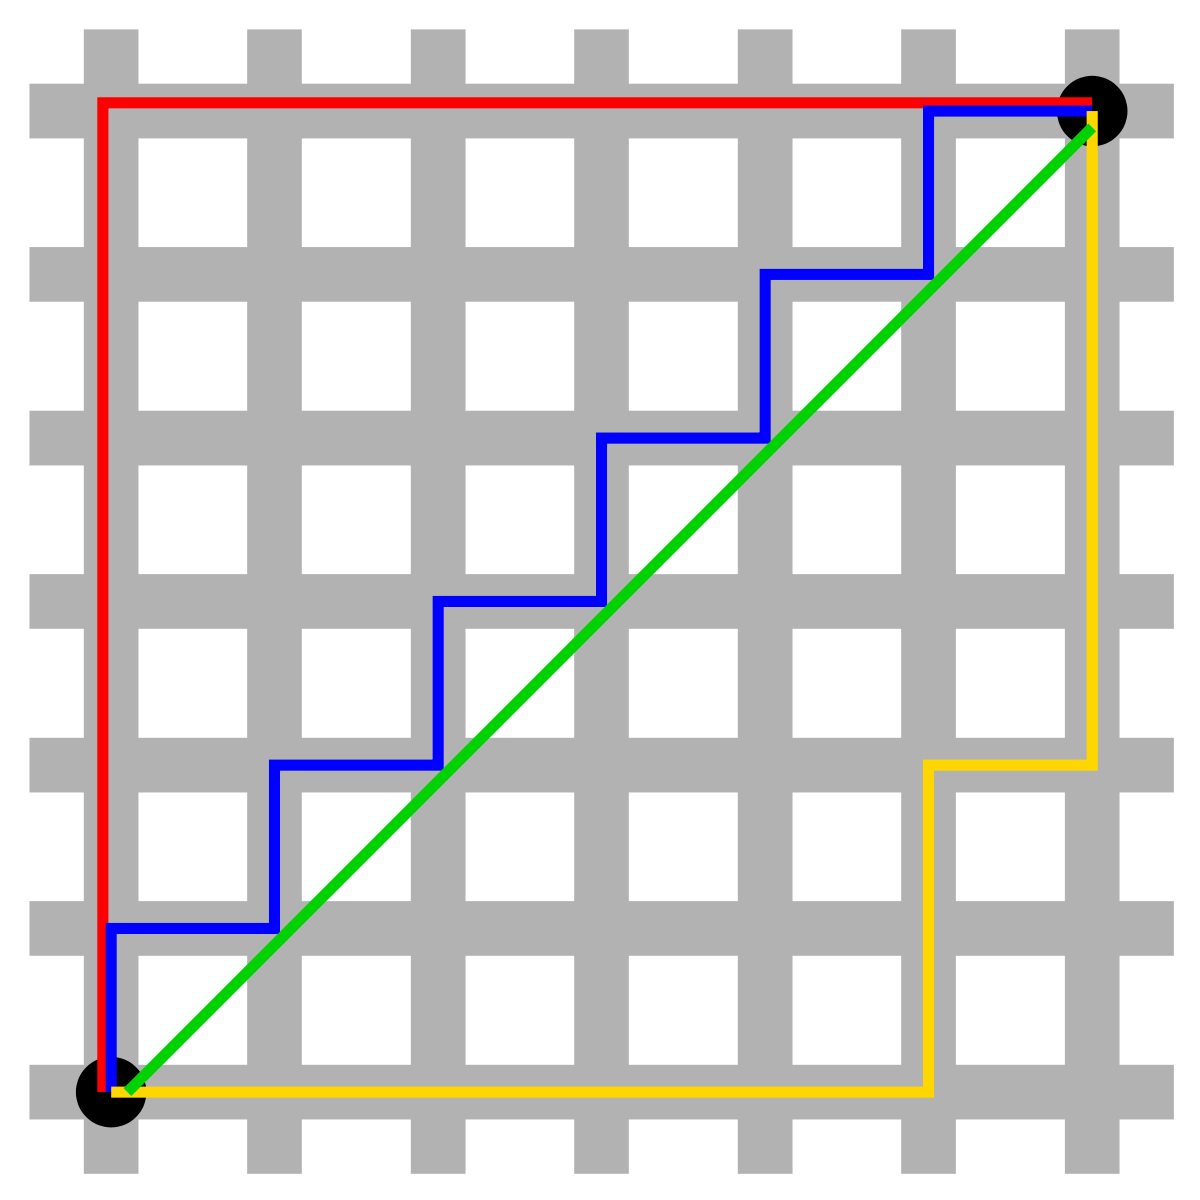
\includegraphics[width=0.15\textwidth, height=0.15\textwidth]{manhattan-distance.png}
\end{wrapfigure}

Algorytmy oceny heurystycznej, które przetestowałem, opierały się na dystansie manhatańskim. W łamigłówce dystans ten jest liczony jako suma różnicy kolumn i różnicy wierszy.
\begin{align*}
    x\_curr & = \textit{kolumna w której znajduje się puzzel układanki} \\
    x\_target &= \textit{kolumna w której powinien znajdować się puzzel układanki} \\
    y\_curr &= \textit{wiersz w której znajduje się puzzel układanki} \\
    y\_target &= \textit{wiersz w której powinien znajdować się puzzel układanki} \\
    \\
    \textit{manhattan distance} &= abs(x\_curr - x\_target) + abs(y\_curr - y\_target)
\end{align*}
\\
\subsection*{Heurystyka 1}
Pierwsza haurystyka zliczała odległości każdego elementu do jego miejsca docelowego.
\[ manhattan(\textit{Puzzle p}) = abs(p.x - p.expected\_x) + abs(p.y - p.expected\_y) \]
\[ h1 = \sum_{p \in Puzzle} manhattan(p) \]

\subsection*{Heurystyka 2}
Druga heurystyka dodaje wagę do każdego dystansu na podstawie kolejności elementów, w taki sposób aby element $1$ w największym stopniu wypływał na wartość, natomiast element $15$ w najmniejszym. Celem takiego zabiegu było nakierowanie przeszukania tak, aby zacząć układać łamigłówkę od lewego-górnego rogu. 
\[ h2 = \sum_{p \in Puzzle} manhattan(p) * (16 - p.value) \]

\subsection*{Heurystyka 3}
Huerystyka 3 wykorzystuje wartość $h2$, natomiast dodaje odległość pustej kratki do pierwszego nie ustawionego na swoim miejscu elementu. Celem było preferowanie rozwiązań, które zbliżają się do ustawienia kolejnego elementu.
\[ h3 = \sum_{p \in Puzzle} \bigg( manhattan(p) * (16 - p.value) \bigg) + manhattan(\textit{first not ordered})\]


\section*{Metodyka testów}
Na początku testu generowana jest prawidłowo ułożona łamigłówka. Następnie jest ona mieszana wykonując $256$ poprawnych ruchów (rozmiar łamigłówki podniesiony do 4 potęgi). W ten sposób zapewnione jest, że łamigłówkę da się rozwiązać.\\
Następnie po kolei uruchamiany jest algorytm $A*$ z odpowiednią wersją algorytmu oceny heurystycznej. Każde uruchomienie rozpoczyna od tej samej łamigłówki początkowej, oraz ma ograniczony czas na rozwiązanie jej - 4 godziny. Z tego też względu nie każdy test zakończył się znalezieniem ścieżki, natomiast można go użyć do wyznaczenia dolnej granicy poszukiwanych wartości, ponieważ rzeczywiste wartości byłyby większe gdyby nie ograniczenia czasowe.
Każdy test został wykonany 10-krotnie.

\renewcommand{\arraystretch}{1.5}
\newcolumntype{M}[1]{>{\centering}m{#1}}

\section*{Wyniki}
\subsection*{Ukończone testy}
\phantom{.}\\
Średnie wartości z testów które ukończyły się we wskazanym czasie.\\

\begin{tabular}{ |M{3.5cm}|M{2cm}|M{2cm}|M{2cm}|c| } 
    \hline
    Wartości & h1 & h2 & h3 & \\
    \hline
    Ilość testów ukończonych w czasie & 8/10 & 3/10 & 9/10 & \\
    \hline
    & 77    & 164    & 186    & mediana \\
    Długość ścieżki & 77.75 & 184.66 & 190.88 & średnia \\
    & 9.24  & 75.72  & 29.26  & odchylenie standardowe \\
    \hline
    & 8549    & 3517    & 5155     & mediana \\
    Liczba odwiedzonych stanów & 8397.25 & 8725.33 & 10643.00 & średnia \\
    & 4449.07 & 8358.31 & 10801.06 & odchylenie standardowe \\
    \hline
    & 15m 23s &  2m 33s & 6m 35s     & mediana \\
    Czas wykonania & 18m 13s & 28m 49s & 43m 49s    & średnia \\
    & 15m 41s & 38m 12s & 1h 12m 44s & odchylenie standardowe \\
    \hline
\end{tabular}

\subsection*{Dolna granica}
\phantom{.}\\
Dolna granica wartości, wliczająca nieukończone testy. Dla testów które nie zakończyły się w czasie, jako długość ścieżki brana jest długość ścieżki (kandydata na rozwiązanie) ostatnio sprawdzanego stanu.\\

\begin{tabular}{ |M{3.5cm}|M{2cm}|M{2cm}|M{2cm}|c| } 
    \hline
    Wartości & h1 & h2 & h3 & \\
    \hline
    & 77    & 155    & 184    & mediana \\
    Długość ścieżki & 78.90 & 166.70 & 186.90 & średnia \\
    & 9.06  & 47.60  & 30.23  & odchylenie standardowe \\
    \hline
    & 9578     & 35364    & 7013     & mediana \\
    Liczba odwiedzonych stanów & 13395.40 & 27639.80 & 13193.20 & średnia \\
    & 10774.49 & 13211.72 & 12787.82 & odchylenie standardowe \\
    \hline
    & 18m 14s    & 4h         & 11m 33s    & mediana \\
    Czas wykonania & 1h 2m 34s  & 2h 56m 38s & 1h 3m 26s  & średnia \\
    & 1h 29m 48s & 1h 39m 1s  & 1h 30m 41s & odchylenie standardowe \\
    \hline
\end{tabular}

\vspace{3cm}

\subsection*{Porównanie}
\phantom{.}\\
Porównanie na mniejszych danych - dla łamigłówki 3x3. Pozwala to na puszczenie większej liczy testów - 100 iteracji na każdą heurystykę.\\

\begin{tabular}{ |M{3.5cm}|M{2cm}|M{2cm}|M{2cm}|c| } 
    \hline
    Wartości & h1 & h2 & h3 & \\
    \hline
                    & 28    & 49    & 52 & mediana \\
    Długość ścieżki & 28.60 & 50.00 & 53.20 & średnia \\
                    & 4.38  & 10.88 & 18.63 & odchylenie standardowe \\
    \hline
                               & 466    & 605    & 253    & mediana \\
    Liczba odwiedzonych stanów & 746.10 & 807.90 & 440.20 & średnia \\
                               & 704.09 & 524.26 & 412.44 & odchylenie standardowe \\
    \hline
                   & 1.2s  & 2.0s & 0.4s & mediana \\
    Czas wykonania & 5.6s  & 5.0s & 1.9s & średnia \\
                   & 10.3s & 5.4s & 2.4s & odchylenie standardowe \\
    \hline
\end{tabular}

\subsection*{Wnioski}
Da się zauważyć bardzo dużą różnorodność w wynikach (odchylenie standardowe jest bardzo duże). Mimo to, korzystając ze średniej oraz mediany można stwierdzić, iż algorytm 1 (najprostszy) pozwala na znalezienie najkrótszej ścieżki (około 77 ruchów przy 256 ruchach mieszających łamigłówkę). Algorytm 2 znajduje ścieżkę dłuższą, jednak nadal krótszą niż pomieszanie łamigłówki (około 190 ruchów przy 256 ruchach mieszających łamigłówkę).
Algorytm 2 jest znacznie dłuższy niż pozostałe 2, ponieważ większość uruchomień sprawdzało ponad 35000 stanów i trwało ponad 4h, mimo to nie znajdując rozwiązania.\\
Ponadto algorytm 1 jest znacznie bardziej stabilny niż algorytm 3. Odchylenie standardowe ilości odwiedzonych stanów algorytmu 1 wynosi 53\%, natomiast algorytmu 3 ponad 101\%.\\
Zatem najlepszym z porównywanych algorytmem oceny heurystycznej jest algorytm 1.
